\documentclass[12pt]{article}
\usepackage{graphicx} % Required for inserting images
\usepackage[letter, margin=0.1in]{geometry}
\usepackage{amsmath}
\usepackage{mathrsfs}
\usepackage{amssymb}
\usepackage[b]{esvect}
\setcounter{secnumdepth}{0} % Removes section numbering

\begin{document}

Galilean Relativity
$$
x = x^{\prime} + vt, y = y^{\prime}, z = z^{\prime}
$$

Time dilation and length contraction
$$
\gamma = \frac{1}{\sqrt{1-\frac{v^2}{c^2}}} \hspace{1cm} t = \gamma t_0 \hspace{1cm} \ell = \frac{\ell_0}{\gamma} \hspace{1cm} v = c \sqrt{1 - (\frac{\ell}{\ell_0})^2} \hspace{1cm} v = c \sqrt{1 - (\frac{t_0}{t})^2}
$$

Lorentz transform
$$
x^{\prime} = \gamma(x-vt) \hspace{2cm} t^{\prime} = \gamma(t-\frac{vx}{c^2}) \hspace{2cm} v_{x}^{\prime} = \frac{v_x - u}{1 - \frac{u v_x}{c^2}}
$$
$$
x = \gamma(x^{\prime} + vt) \hspace{2cm} t = \gamma(t^{\prime} + \frac{vx^{\prime}}{c^2}) \hspace{2cm} v_{x} = \frac{v_x^{\prime} + u}{1 + \frac{u v_x^{\prime}}{c^2}}
$$

Doppler effect, f: f of observer, $f_0$: f of rest frame of source

$$
f_{towards} = \sqrt{\frac{c + v}{c - v}}f_o \hspace{2cm} f_{away} = \sqrt{\frac{c - v}{c + v}}f_o
$$

Relativistic momentum

$$
\Vec{p} = \gamma m \Vec{v}  \hspace{0.5cm} m_{rel} = \gamma m_{rest} \hspace{0.5cm} p_{photon} = \frac{E}{c} = \frac{hf}{c} = \frac{h}{\lambda}
$$

Relativistic Energy
$$
E^2 = (pc)^2 + (mc^2)^2 \hspace{0.5cm} E = 
hf = \frac{hc}{\lambda} \hspace{0.5cm} E = K + mc^2 \hspace{0.5cm} K = (\gamma - 1) mc^2 \hspace{0.5cm} E = \frac{p^2}{2m} \hspace{0.5cm} E_{tot} = \gamma mc^2$$

Speed of light
$$
c = \frac{1}{\sqrt{\epsilon_0 \mu_0}} = \lambda f = \frac{d}{t}
$$

Black Body Law I: Intensity, $\sigma$: constant, T: \underline{Absolute} temperature
$$
I = \sigma T^4
$$

Einstein's Photoelectric Effect Work Function
$$
K = hf - \phi \rightarrow K_{max} = \frac{1}{2}mv_{max}^2 \hspace{0.5cm} \boldsymbol{e V_0} = hf - \phi, 
$$

Bremsstrahlung, only for x-ray production, $V_AC$: Accelerating voltage.
$$
e V_{AC} = hf_{max} = \frac{hc}{\lambda_{min}}
$$

Compton Scattering
$$
\lambda^{\prime} - \lambda = \frac{h}{mc}(1-cos(\phi)) \rightarrow \lambda^{\prime}_{max} = \lambda + 2 \frac{h}{mc}
$$

Heisenberg Uncertainty Principle
$$
\Delta x \Delta p_x \geq \frac{\hbar}{2} \hspace{2cm} \Delta t \Delta E \geq \frac{\hbar}{2}
$$

$$
p_x = \frac{h}{\lambda} = \frac{h}{2\pi} \frac{2\pi}{\lambda} = \hbar k
$$

$$
E = hf = \frac{h}{2\pi} 2 \pi f = \hbar \omega
$$

\newpage

\centering{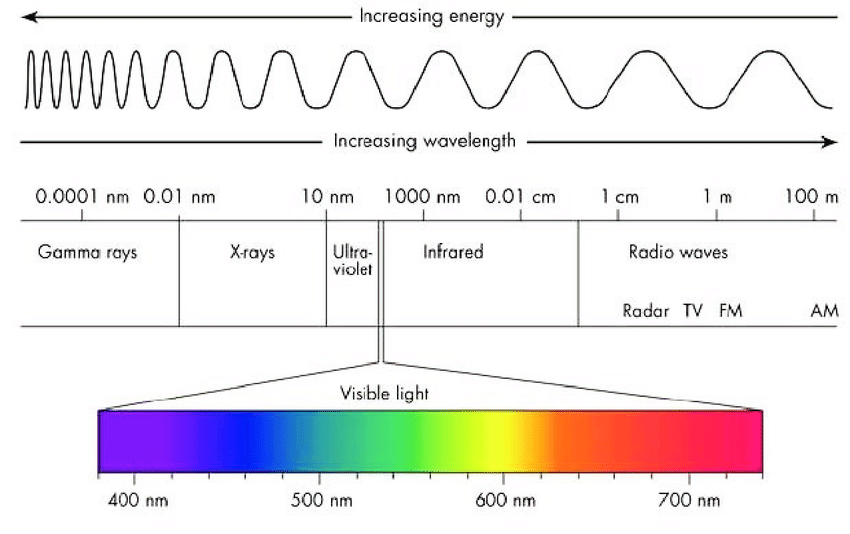
\includegraphics[scale=0.65]{EMSpec}}
\centering{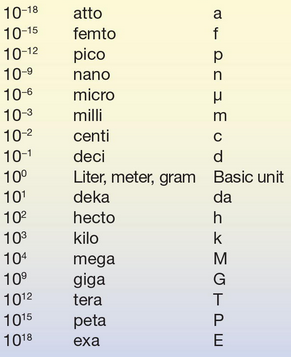
\includegraphics[scale=1]{SIPrefixes}}

Constants
$$
h = 6.626 \times 10^{-34} J \cdot s, \hbar = \frac{h}{2 \pi}
$$
$$
\epsilon_0 = 8.854 \times 10^{-12} F \cdot m^{-1}
$$
$$
\mu_0 = 1.256 \times 10^{-6} N \cdot A^{-2}
$$
$$
\sigma = 5.670 \times 10^{-8} W \cdot m^{-2} \cdot K^{-4}
$$
$$
m_{p} = 1.672 \times 10^{-27} kg
$$
$$
m_{e} = 9.109 \times 10^{-31} kg
$$
$$
eV = 1.602 \times 10^{-19} C
$$
$$
c = 3.00 \times 10^{8} \frac{m}{s}
$$




\end{document}
